\documentclass[english]{sig-alternate}
\usepackage{color}
\usepackage{xcolor}
\usepackage{colortbl}
\usepackage{amstext}
\usepackage{pdfpages}
\usepackage{alltt}
\usepackage{epstopdf}
\usepackage{listings}
\lstset{basicstyle=\ttfamily,breaklines=true}
\usepackage{xspace,colortbl}
\usepackage[USenglish]{babel}
\usepackage{multirow}
\usepackage{url}
\usepackage{subfigure}
\usepackage{graphicx}
\usepackage{amssymb}
\usepackage{fmtcount}
\usepackage{amsfonts}
\usepackage{xspace}
\usepackage{amsmath}
\usepackage{multirow}
\usepackage[mathscr]{eucal}
\usepackage{times}
\usepackage{colortbl}
\usepackage{bm}
\usepackage[nospace]{cite}
\makeatletter
\newif\if@restonecol
\makeatother
\let\algorithm\relax
\let\endalgorithm\relax
\usepackage[lined,boxed,vlined,ruled]{algorithm2e}
\special{papersize=8.5in,11in}



\setcounter{secnumdepth}{3}

\long\def\comment#1{}
%\usepackage[dvipdfm]{hyperref}
%\usepackage[dvips]{hyperref}
\begin{document}
%\conferenceinfo{SIGMOD'14,} {June 22--27, 2014, Snowbird, Utah, USA.}
%\CopyrightYear{2014}
%\clubpenalty=10000
%\widowpenalty = 10000

%\hyphenpenalty=5000
\tolerance=1000
\linespread{1}%
%\pagenumbering{arabic}

\title{Deep Clearning: Declarative Big Data Cleaning} 


\iffalse
\author{\alignauthor Sanjay Krishnan,~~Jiannan Wang,~~Sameer Agarwal,~~Michael J. Franklin,~~Ken Goldberg \\
\vspace{.2em}\affaddr{AMPLab, UC Berkeley} \\
\fontsize{9}{10}\selectfont\ttfamily\upshape
\vspace{.1em}\{sanjay,jnwang\}@eecs.berkeley.edu, \{sameerag,franklin\}@cs.berkeley.edu, goldberg@berkeley.edu
}
\fi

\newcommand{\squishlist}{
   \begin{list}{$\bullet$}
    { \setlength{\itemsep}{0pt}
      \setlength{\parsep}{2pt}
      \setlength{\topsep}{6pt}
      \setlength{\partopsep}{0pt}
      \leftmargin=5pt
\rightmargin=0pt
\labelsep=5pt
\labelwidth=10pt
\itemindent=0pt
\listparindent=0pt
\itemsep=\parsep
    }
}
\newcommand{\squishend}{\end{list}}

%\linespread{0.96}


%Identifying Similarity Functions from Examples for Effective Record Matching

%\subtitle{[Extended Abstract]
%\titlenote{A full version of this p aper is available as
%\textit{Author's Guide to Preparing ACM SIG Proceedings Using
%\LaTeX$2_\epsilon$\ and BibTeX} at
%\texttt{www.acm.org/eaddress.htm}}}
%\pagenumbering{arabic}

\newtheorem{theorem}{Theorem}
\newtheorem{example}{Example}
\newtheorem{definition}{Definition}
\newtheorem{proposition}{Proposition}
\newtheorem{lemma}{Lemma}
\newtheorem{corollary}{Corollary}
\newtheorem{demonstration}{Demonstration}

\newcommand{\dataset}{data set\xspace}
\newcommand{\datasets}{data sets\xspace}
\newcommand{\biascorrected}{NormalizedSC\xspace}
\newcommand{\bias}{\biascorrected}
%\newcommand{\sampledirty}{\texttt{SampleDirty}\xspace}
%\newcommand{\sampleclean}{\texttt{SampleClean}\xspace}
%\newcommand{\allclean}{\texttt{AllClean}\xspace}
%\newcommand{\alldirty}{\texttt{AllDirty}\xspace}
\newcommand{\sampledirty}{{SampleDirty}\xspace}
\newcommand{\sampleclean}{{RawSC}\xspace}
\newcommand{\allclean}{{AllClean}\xspace}
\newcommand{\alldirty}{{AllDirty}\xspace}
\newcommand{\sys}{\textsf{DeepClearner}\xspace}
\newcommand{\projx}{\sys}
\newcommand{\saqp}{SAQP\xspace}
\newcommand{\saqpplus}{\projx}
\newcommand{\blinkdb}{BlinkDB\xspace}
\newcommand{\ctable}{\ensuremath{T^{clean}}\xspace}
\newcommand{\var}{\ensuremath{\texttt{var}}\xspace}

\newcommand{\attr}[1]{\texttt{#1}\xspace}
\newcommand{\afunc}[1]{\texttt{#1}\xspace}
\newcommand{\M}{\ensuremath{M}\xspace}
\newcommand{\Pset}{\ensuremath{P}\xspace}
\newcommand{\gfunc}{\ensuremath{f}\xspace}
\newcommand{\avgfunc}{\ensuremath{\texttt{avg} }\xspace}
\newcommand{\varfunc}{\ensuremath{\texttt{var} }\xspace}
\newcommand{\productfunc}{\ensuremath{\texttt{product} }\xspace}
\newcommand{\geomeanfunc}{\ensuremath{\texttt{geomean} }\xspace}
\newcommand{\countfunc}{\ensuremath{\texttt{count} }\xspace}
\newcommand{\sumfunc}{\ensuremath{\texttt{sum} }\xspace}
\newcommand{\groupby}{\ensuremath{\texttt{group-by}}\xspace}
\newcommand{\PCset}{\ensuremath{P^{(c)}}\xspace}
\newcommand{\PCseti}[1]{\ensuremath{P^{(c)}_{#1}}\xspace}
\newcommand{\SCset}{\ensuremath{S}\xspace}
\newcommand{\Sset}{\ensuremath{S}\xspace}
\newcommand{\Pseti}[1]{\ensuremath{P_{#1}}\xspace}
\newcommand{\Sseti}[1]{\ensuremath{S_{#1}}\xspace}
\newcommand{\di}[1]{\ensuremath{d_{#1}}\xspace}

\newcommand{\Correct}[1]{\texttt{Correct}\ensuremath(#1)\xspace}
\newcommand{\Remove}[2]{\texttt{Remove}\ensuremath(#1, #2)\xspace}
\newcommand{\Predicate}[1]{\texttt{Predicate}\ensuremath(#1)\xspace}
\newcommand{\Dedup}[2]{\texttt{Dedup}\ensuremath(#1)\xspace}


\def\indistHIGH{\,{\buildrel d \over \rightarrow}\,} 

\newcommand{\reminder}[1] {{{\bf [[[#1]]]}\xspace}}
%\newcommand{\reminder}[1] {}


\newcommand{\ewu}[1]{\noindent{\color{blue}{EWu: #1}}}
\newcommand{\sanjay}[1]{\noindent{\color{red}{SanJ: #1}}}
\newcommand{\haas}[1]{\noindent{\color{red}{Haas: #1}}}
\newcommand{\team}[1]{\noindent{\color{red}{Haas or SanJ: #1}}}
\newcommand{\jn}[1]{\noindent{\color{red}{JW: #1}}}


\pagestyle{plain}





\maketitle
\thispagestyle{plain}



% A category with the (minimum) three required fields
%\category{H.4}{Information Systems Applications}{Miscellaneous}
%A category including the fourth, optional field follows...
%\category{D.2.8}{Software Engineering}{Metrics}[complexity measures, performance measures]
%\terms{Delphi theory}
%\keywords{ACM proceedings, \LaTeX, text tagging}

% !TEX root = demo.tex
\begin{abstract}
%The prevalence of dirty data presents a fundamental obstacle to modern data-driven applications.
Analysts report spending upwards of 80\% of their time on problems in data cleaning.
The data cleaning process is inherently iterative, with evolving cleaning workflows that 
start with basic exploratory data analysis on small samples of dirty data, then refine analysis with 
more sophisticated/expensive cleaning operators (e.g., crowdsourcing), and finally apply the insights to a full dataset.
While an analyst often knows at a logical level what operations need to be done, they often have 
to manage a large search space of physical operators and parameters.
We present \sys, a system designed to support the iterative development and optimization of data cleaning workflows, especially ones that utilize the crowd.
\sys separates logical operations from physical implementations, and driven by analyst feedback, suggests optimizations and/or replacements to the analyst's choice of physical implementation.
We highlight research challenges in sampling, in-flight operator replacement, and crowdsourcing. 
We overview the system architecture and these techniques, 
then provide a demonstration designed to showcase how \sys can improve iterative data analysis
and cleaning. 
The code is available at: \url{http://www.sampleclean.org}.
\end{abstract}


% !TEX root = demo.tex
\section{Introduction}\label{sec:intro}

\begin{figure}[t]
\centering
\vspace{-0.5cm}
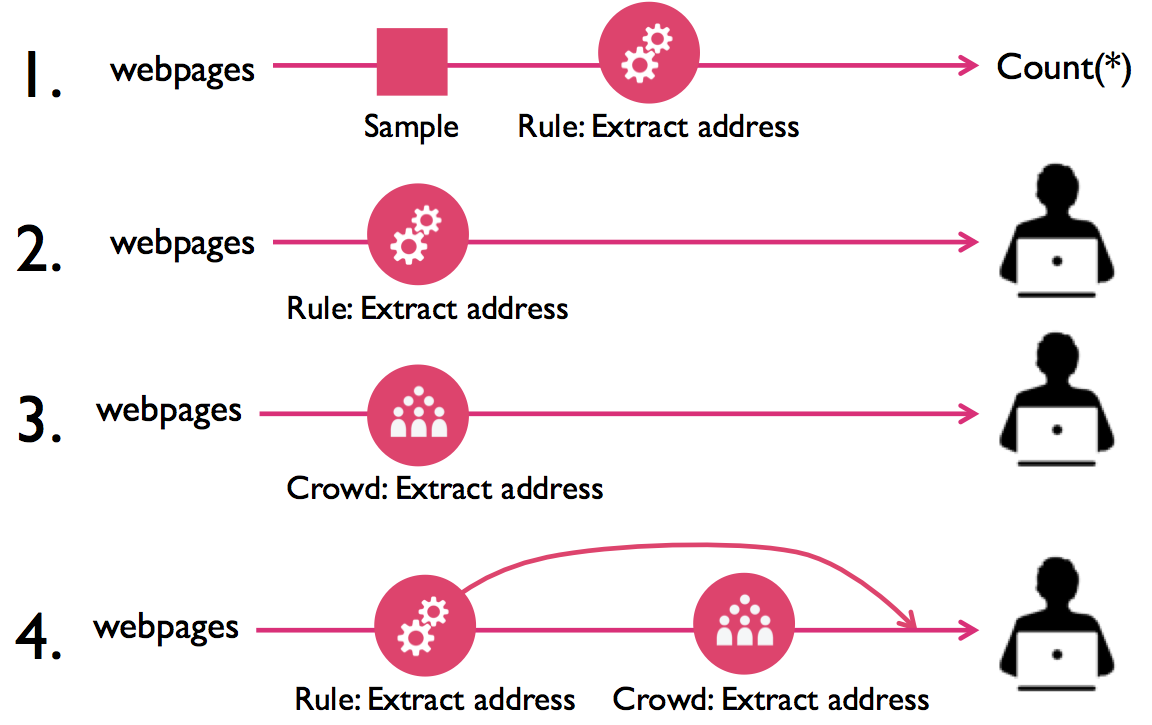
\includegraphics[width = .4\textwidth]{figs/lifecycle.png}
\vspace{-0.4cm}
\caption{Example iterations on the design of the portion of a cleaning plan that extracts restaurant addresses from their unstructured webpages.  
1) An exploratory plan that uses a sample to evaluate a simple address extraction method.
2) A plan that applies the method to the entire dataset. The quality is unsatisfactory. 
3) An alternate plan that uses manual crowd extraction. The quality is now high, but the crowd-based extractor is slow. 
4) A hybrid plan that sends only difficult webpages to the crowd, maximizing accuracy without sacrificing latency.}
\label{fig:ex-plan}
\vspace{-0.3cm}
\end{figure}
% why feedback loops exist/are important (cite Joe’s shit in the past 3 years, blinkdb, etc.). highlight domain specificity. Large variety of data cleaning tasks

%
% General comment that data cleaning is important:
%
The ease of acquiring and merging many large-scale data sources has led to a prevalence of dirty data.
Unfortunately, blindly using results that are derived from dirty data can lead to hidden yet significant errors in modern data-driven applications, so data must be cleaned before it is used.
But because data cleaning is often specific to the domain, dataset, and eventual analysis, analysts report spending upwards of 80\% of their time on problems in data cleaning~\cite{kandel2012}.
The analyst is faced with a breadth of possible errors that are manifest in the data and a variety of options to resolve them.
She must go through the cleaning process via trial and error, deciding for each of her data sources what to extract, how to clean it, and whether that cleaning will significantly change results.

Data cleaning is inherently iterative and Figure~\ref{fig:ex-plan} shows a common progression for the development of a data cleaning plan, in this case the extraction of a restaurant's address from its unstructured webpage.
While this operation can easily be represented at a \textit{logical} level by its input and output schema, there is a huge space of possible \textit{physical} implementations of the logical operators. 
For example, extraction could depend on manually specified rules (\textit{rule-based}), use models trained on previously extracted ground truth records (\textit{learning-based}), ask crowd workers to extract the desired data fields (\textit{crowd-based}), or some combination of the three (e.g., active learning, which uses crowd workers to provide labels for a learning-based approach).
Even after selecting (say) a crowd-based operator, many parameters might influence the quality of the output data or the speed and cost of cleaning: the number of crowd workers who vote on the extraction for a given webpage, the amount each worker is paid, etc.
A priori, a data analyst has little intuition for what physical plan will be optimal in this large space.

Note that in the evolution of the data cleaning plan in Figure~\ref{fig:ex-plan}, our data analyst needed to make many decisions manually about the choice of physical operators by reasoning about their latency, accuracy, and cost. 
Making the wrong decision, for example using the crowd when it only marginally improves accuracy, can be very costly.
A general, scalable, and interactive system that supports rapid iteration on candidate plans would greatly aid this process.

%The prevalance of data cleaning systems in both the research and industrial communities --
%Corleone does blah, XXX addresses blah. Nadeef does blah -- speak to the importance of a
%data cleaning framework as part of the modern big data ecosystems. \ewu{include open access of data in argument?} \jn{We also need to take a look at data cleaning systems in industry. }


% why existing systems suck aka related work
% 1. have slow feedback loops (dataset-dependence, …)
% 2. solve very specific data-cleaning tasks
%Since the beginning of data management, systems have been explored by both the research and industrial communities to improve data cleaning efficiency and quality.
Existing systems seldom address the end-to-end iterative data cleaning process described above.
Extract-transform-load (ETL) systems~\cite{informatica,talend,apachefalcon} require developers to manually write data cleaning rules and execute them as long batch jobs, 
and constraint-driven tools allow analysts to define ``data quality rules" and automatically propose corrections to maximally satisfy these rules \cite{DBLP:conf/sigmod/DallachiesaEEEIOT13}.
Unfortunately, neither provide the opportunity for iteration or user feedback, inhibiting the user's ability to rapidly prototype different data cleaning solutions.
Projects such as Wrangler~\cite{wrangler,trifacta} and OpenRefine~\cite{openrefine} support iteration with spreadsheet-style interfaces that enable the user to compose data cleaning sequences by directly manipulating a sample of the data and applying these sequences to the full dataset.
However, they are limited to specific cleaning tasks such as simple text transformations, do not support crowd-based processing at scale, and cannot incorporate user feedback to optimize the physical implementation of the data cleaning sequences.
Crowd-based~\cite{gokhale2014corleone,stonebraker2013data} systems have been proposed to relieve the data analyst of the burden of rule specification or manual cleaning, but are usually specific to a single cleaning task (e.g.,~\cite{gokhale2014corleone,park2014crowdfill,eracer,chen2014integrating}), preventing end-to-end optimization of the entire cleaning plan.
These existing limitations suggest the need for a system that is general enough to adapt to a wide range of data cleaning applications, scales to large datasets, and natively supports fast-feedback interactions to enable rapid data cleaning iteration.

In this paper, we introduce \sys, a system designed to support the iterative development and optimization of data cleaning plans end to end.
\sys allows users to specify declarative data cleaning plans composed of rule-based, learning-based, or crowd-based operators, then iterate rapidly on plans with cost-aware recommendations for improving the accuracy or latency of a plan.
The effects of a plan can be viewed early using sampling and approximate query processing techniques~\cite{wang1999sample}.

Supporting these capabilities requires a combination of careful engineering 
as well as tackling several research challenges:

\squishlist
\item \textbf{Sampling}: We provide sampling as a first-class logical operator for data cleaning plans that tolerate approximation, and use it to speed up iteration on early-stage plans.

\item \textbf{Recommendation}: We recommend cost-aware changes to in-flight cleaning plans that allow users to trade off accuracy and latency, and provide efficient mechanisms for implementing recommended changes without re-executing the plan on already cleaned tuples.

\item \textbf{Crowd Latency}: We leverage techniques for straggler mitigation~\cite{venkataraman2014power} and model crowd worker speed and accuracy to reduce the (often rate-limiting) latency of crowd data cleaning, consistently retrieving results in seconds rather than hours.
\squishend

In our demonstration, we will run an entity resolution plan on two restaurant datasets, and
show how \sys can be used to 1) specify, modify, and execute a data cleaning plan,
2) quickly clean a sample to characterize how a plan is performing, and
3) observe the same cleaning plans running on multiple datasets.
Users can execute plans over a live crowd that uses the audience as workers, or a simulated crowd
that uses pre-collected crowd responses. The dashboard (Figure~\ref{screenshot}) also provides a live inspection
interface to view the status of the cleaning plan as it executes.

\vspace{-0.2cm}
%Our contributions/requirements
%different ways to tighten the feedback loop:
%end-to-end latency/cost (operator optimization)
%looking versus touching
%Adding introspection (more points of observation)
%hot-swapping (more points of changing plans)
%We have built an end-to-end data cleaning framework with these requirements in mind. (... things we do …) (... engineering contributions …).
%In this demonstration, we highlight the benefits of improving feedback loops for data cleaning using X datasets by optimizing a data cleaning pipeline for one data set/cleaning task, then quickly fitting the pipeline to another dataset.


\if{0}

\jn{Honestly, I didn't quite buy declarativity of the system. In my opinion, data cleaning is so domain specific. It's hard to make it declarative. For a given domain, people may need to write their own data cleaning system. There is a lack of a data cleaning framework that they can build based on. This motivates us to develop such framework. 


We analyze a large variety of domain specific data cleaning systems, and identify several key components: declarative data cleaning operators (e.g., similarity joins), active learning, and crowd/expert sourcing platforms that they require. In our framework, we abstract these components, and implement them in a general way. 

We mainly address two challenges: extensibility and scalability. For the former one, we came up with a nice data-cleaning pipeline API, which people can easily use to compose their own data cleaning tasks. For the latter one, we address it in two aspects: Sampling + Asynchrony.}

\ewu{That's fair, will need to address why a framework is necessary and what benefits it provides.  I think a framework is the correct pitch, hard to sell a set of operators.  Are the above challenges -- extensibility and scalability -- actually difficult?  Worried it's straightforward application of existing techniques.}



In contrast, our work is based on the observation that the majority of data cleaning workflows
can be decomposed into a small set of logical operations (in addition to traditional database operators):
filter based on constraints, extract new fields from existing data, and a similarity join to match
similar or duplicate records. \ewu{quickly validate why this observation holds.} \jn{Yes! I also found that Sec 2.3 has more operators than you describe here.}  
By designing a system around these core operators, we can provide a vast library of physical  
data cleaning operators that span the range of algorithmic, machine learning, and human computation-based
implementations that are necessary practical data cleaning pipelines.   \ewu{Describe live inspection as 
a core feature or is it too easy?}

Designing such a system requires tackling several design challenges:

\begin{enumerate}
\item Speed
\item Quality
\item API Design/extensibilty
\end{enumerate}



We have implemented an initial version of \sys on top of the AMPLab Spark stack, which provides us 
with access to its advanced distributed processing and machine learning features.  Our goal for the current
version is to implement the core mechanisms for declarative specification of the
data cleaning pipeline, solidify the API design, and incle support for, and implementations of,
multiple classes of physical data cleaning operators.


\fi



\if{0}

Cleaning, pre-processing, and formatting data is a required first step in any data analytics pipeline.
However, despite this importance, large-scale data analytics platforms such as Spark or Hadoop lack integrated data cleaning frameworks.
There are a few challenges in building a general purpose data cleaning framework: (1) data cleaning is often
domain specific and requires specialized software targeted at one or a handful of data sources \cite{wang1999sample}, (2) data cleaning is often 
expensive as it increasingly involves human effort via crowdsourcing or experts \cite{DBLP:conf/sigmod/GokhaleDDNRSZ14}, and (3) learning how to clean dirty data from examples
is often hard without a greatly restricted set of operators \cite{DBLP:conf/uist/GuoKHH11}.

We address this problem in \projx by designing a Spark library of composable and scalable data cleaning primitives.
\projx abstracts the logical data cleaning operators: Extraction, Similarity Join, Filtering, from the physical implementation i.e, Rule, Crowd, or Machine Learning.
We interface these primitives through a DSL with which a user can build data cleaning operators that suit their needs.
\projx provides transparent optimizations for each of the components and their composition.
In this demonstration proposal, we present \projx and highlight some of its key features.
While there are many existing systems that do one aspect of data cleaning and transformation (e.g Entity Resolution or Extraction), 
many real world data cleaning tasks have multiple types of errors.
Composing disparate systems can lead to complex code and inefficiencies at scale.
With \projx, we hope to design a set of optimized composable primitives that span a large space of data cleaning tasks.

The first key feature of \projx is that it provides optimized distributed implementations 
of the physical data cleaning operators.
For example, a key step in many deduplication algorithms is a Similarity Join which finds all pairs of records that are within some similarity threshold.
A naive implementation of a Similarity Join would apply a similarity function to all pairs of records.
However, in \projx, we provide optimized implementations of certain common similarity functions (e.g Jaccard, Edit Distance, etc.) that allow for 
a combined broadcast join and prefix filtering which intelligently skips pairs of records using a broadcasted inverted index.

Another feature of \projx is managing the latency and the scale problems of crowd-based data cleaning. 
Crowdsourcing is increasingly prevalent in data cleaning, and \projx provides physical crowd-based implementations
of the logical operators.
However, crowds work at a different latency and scale point in comparison to distributed analytics platforms.
To address the latency problem, we build asychrony into the system.
The user can query intermediate results at any time as crowd responses stream in.
To address the scale issue, \projx provides sampling primitives.
The glue that ties all of the crowd components together is a Machine Learning technique called Active Learning.
As we collect more and more crowd responses, we learn a model that predicts these responses to apply it on the uncleaned data.
Active Learning selects the most informative questions to ask the crowd.

Finally, \projx provides an approximate query processing (AQP) framework.
With slow asynchronous data cleaning algorithms as in crowdsourcing, we need 
to define clear semantics for the intermediate results.
Our AQP framework uses the algorithms proposed in \cite{wang1999sample}, to estimate and bound early results.
It is also common for data scientists to prototype expensive data cleaning pipelines on samples and AQP allows quick evaluation of
aggregate query results on a cleaned sample.

\subsection{Demonstration Scenario}
\reminder{TODO}

\fi




\if{0}
Consider for example, the ability to rapidly understand the types of errors that are present, as well as prevalance of 
these errors is cruicial.



Before an organization can use a new dataset as part of their analysis pipeline
(e.g., to build complex learning models or answer analyst queries)
the errors in the dataset need to be removed in order to ensure accurate conclusions.  

Modern data-driven organizations rely on the ability to ingest and generate large data sets from 
disparate sources, and combine the data together to build complex models or answer analytical questions.  
For example, a restaurant review website may collect restaurant listings by scraping data from webpages or purchasing them from external sources, and
restaurant visitation information for sources such as OpenTable or FourSquare, and aggregate the data to
model user eating habits.  
The set of cleaning tasks necessary for each of these data sources is highly domain and application specific,
and oftentimes the developer is concurrently trying to clean the data source as well as understand its properties.


Oftentimes, these data sources have data quality issues that require a complex data cleaning pipeline -- 
e.g., data extraction, re-formatting, identification and fixes of missing or incorrect values,
and removal of redundant information -- before the data is useable by downstream processes.
Data sources are often domain specific and new for the data analyst, 
As datasets continue to grow, and organizations make use of mure and more datasets, the ability to
rapidly clean the data is more important.  
\fi

\vspace{-1em}
\section{Framework Overview}\label{sec-arch}
In this section, we formalize the two main problems that \svc addresses: (1) cleaning the staleness errors in a sample of a MV and (2) answering an aggregate query with a clean sample.

\subsection{Notation and Definitions}\label{notation}
In \svc, we explore the problem of approximate aggregate query processing on stale materialized views using a data cleaning approach.
We assume that these materialized views are periodically maintained and thus are stale in between maintenance periods.
The focus of this paper is analytic workloads where the typical query is a group by aggregate on relatively large views.
\svc provides a framework for increased query accuracy for a flexible additional maintenance cost that can scale with system constraints.

%\reminder{You have defined $\mathcal{D}$, $\{R_i\}$, etc in Definition 1. Maybe you can move Def 1 to this Section?}
\noindent \textbf{Materialized View:} Let $\mathcal{D}$ be a database which is a collection of relations $\{R_i\}$. A \emph{materialized view} $S$ is the result of applying a \emph{view definition} to $\mathcal{D}$. 
View definitions are composed of standard relational algebra expressions: Select ($\sigma_{\phi}$), Project ($\Pi$), Join ($\bowtie$), Aggregation ($\gamma$), Union ($\cup$), Intersection ($\cap$) and Difference ($-$). 
We use the following parametrized notation for joins, aggregations and generalized projections:
\begin{itemize}[noitemsep] \sloppy
	\item $\Pi_{a_1,a_2,...,a_k}(R)$: Generalized projection selects attributes $\{a_1,a_2,...,a_k\}$ from $R$, allowing for new columns that are arithmetic transformations of attributes (e.g., $a_1+a_2$).
	\item $\bowtie_{\phi (r1,r2)}(R_1,R_2)$: Join selects all tuples in $R_1 \times R_2$ that satisfy $\phi (r_1,r_2)$. We use $\bowtie$ to denote all types of joins even extended outer joins such as $\rightouterjoin,\leftouterjoin,\fullouterjoin$.
	\item $\gamma_{f,A}(R)$: Apply the aggregate function $f$ to the relation R grouped by the distinct values of $A$, where $A$ is a subset of the attributes.  
	The DISTINCT operation can be considered as a special case of the Aggregation operation. 
\end{itemize}
The composition of the unary and binary relational expressions can be represented as a tree, which is called the \emph{expression tree}.
At the leaves of the tree are all of the \emph{base relations} for a view.
Each node of the tree is the result of applying one of the above relational expressions to a relation.
To avoid ambiguity, we refer to tuples of the base relations as \emph{records} and tuples of derived relations as \emph{rows}.

\noindent \textbf{Primary Key: } We assume that each of the base relations has a \emph{primary key}. If this is not the case, we can always add an extra column 
that assigns an increasing sequence of integers to each record.
For the defined relational expressions, every row in a materialized view can be also be given a primary key \cite{DBLP:journals/vldb/CuiW03, DBLP:conf/sigmod/ZengGMZ14},
which we will describe in Section \ref{sampling}. 
This primary key is formally a subset of attributes $u \subseteq \{a_1,a_2,...,a_k\}$ such that all $s \in S(u)$ are unique.
We denote the entire row for that primary key as a selection $\sigma_u(S)$.

\vspace{.25em}

\noindent \textbf{Staleness: } For each relation $R_i$ there is a set of insertions $\Delta R_i$ (modeled as a relation)
and a set of deletions $\nabla R_i$.
An ``update'' to $R_i$ can be modeled as a deletion and then an insertion.
We refer to the set of insertion and deletion relations as ``delta relations" denoted by $\partial \mathcal{D}$:
\[
	\partial \mathcal{D} = \{\Delta R_1,...,\Delta R_k\} \cup \{\nabla R_1,...,\nabla R_k\}
\]
A view $S$ is considered \emph{stale} when there exist insertions or deletions to any of its base relations.
This means that at least one of the delta relations in $\partial \mathcal{D}$ is non-empty.

\vspace{.25em}

\noindent \textbf{Maintenance: } There may be multiple ways (e.g., incremental maintenance or recomputation) to maintain a view $S$, and we denote the up-to-date view as $S'$.
We formalize the procedure to maintain the view as a \emph{maintenance strategy} $\mathcal{M}$.
A maintenance strategy is a relational expression the execution of which will return $S'$.
It is a function of the database $\mathcal{D}$, the stale view $S$, and all the insertion and deletion relations $\partial \mathcal{D}$. 
In this work, we consider maintenance strategies composed of the same relational expressions as materialized views described above.
\[
S' = \mathcal{M}(S,\mathcal{D}, \partial D)
\]

\vspace{.25em}

\noindent \textbf{Staleness as Data Error: } The consequences of staleness are incorrect, missing, and superfluous rows. 
Formally, for a stale view $S$ with primary key $u$ and an up-to-date view $S'$:
\begin{itemize}[noitemsep] \sloppy
	\item \textbf{Incorrect: } Incorrect row errors are the set of rows (identified by the primary key) that are updated in $S'$: \[\{\forall u \in S : (\exists u \in S' \wedge (\sigma_u(S) \ne \sigma_u(S')))\}\]
	\item \textbf{Missing: } Missing row errors are the set of rows (identified by the primary key) that exist in the up-to-date view but not in the stale view: \[\{\forall u \in S' : \not \exists u \in S\}\]
	\item \textbf{Superfluous: } Superfluous row errors are the set of rows (identified by the primary key) that exist in the stale view but not in the up-to-date view : \[\{ \forall u \in S : \not\exists u \in S' \}\]
\end{itemize}

\vspace{.25em}

\iffalse
\begin{figure}[t] \vspace{-2em}
\centering
 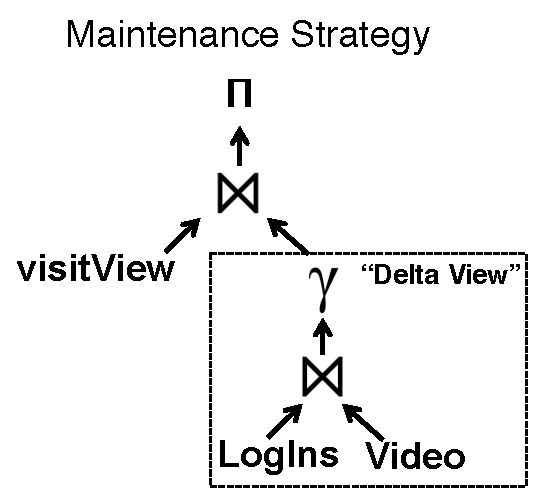
\includegraphics[scale=0.32]{figs/example_expression_tree.pdf} \vspace{-.5em}
 \caption{\reminder{(1). the view definition is different from the one in Sec 2.1; (2) Even if they are the same, it seems not necessary to show it again; (3) Right now you have (b) to show maintenance strategy; maybe you can replace (a) with a figure that shows primary key and ``staleness ad data error"} For our example, we represent the expression tree of the maintenance strategy. We first calculate a delta view using the new insertions and then join this view with the old view.\label{exexpr}}\vspace{-1.5em}
\end{figure}

\vspace{0.45em}
\fi

\noindent \textbf{Uniform Random Sampling: }
We define a sampling ratio $m\in [0,1]$ and for each row in a view $S$, we include it into a sample with probability $m$.
We use the ``hat'' notation (e.g., $\widehat{S}$) to denote sampled relations and sampled relational expressions.
We say the relation $\widehat{S}$ is a \emph{uniform sample} of $S$ if
\[\text{(1) } \forall s \in \widehat{S} : s \in S\text{;~~~~~ (2) }Pr(s_1 \in \widehat{S}) =  Pr(s_2 \in \widehat{S}) = m\]
We say a sample is \emph{clean} if an only if it is a uniform random sample of the up-to-date view $S'$. 

\vspace{0.25em}

\begin{example}\label{concepts}
In this example, we summarize all of the key concepts and terminology pertaining to materialized views, stale data error, and maintenance strategies.
Our example view, visitView, joins the Log table with the Video table and counts the visits for each video grouped by videoId.
Since there is a foreign key relationship between the relations, this is just a visit count for each unique video with additional attributes. 
The primary keys of the base relations are: sessionId for Log and videoId for Video.

If new records have been added to the Log table the visitView is considered stale.
Incorrect rows in the view are videos for which the visitCount is incorrect and missing rows are videos that had not yet been viewed once at the time of materialization. 
While not possible in our running example, superfluous rows would be videos whose Log records have all been deleted.
Formally, in this example our database is $\mathcal{D}=(Video, Log)$, and the delta relations are $\partial\mathcal{D}=(LogIns)$. 

Suppose, we apply the change-table IVM algorithm proposed in \cite{gupta1995maintenance}:
\vspace{-.55em}
\begin{enumerate}[noitemsep]
\item Create a ``delta view" by applying the view definition to LogIns. That is, calculate the visit count per video on the new logs:
\[
 \gamma(Video \bowtie LogIns)
\]
\item Take the full outer join of the ``delta view" with the stale view visitView (equality on videoId).
\[
 VisitView \fullouterjoin \gamma(Video \bowtie LogIns)
\]
\item Apply the generalized projection operator to add the visitCount in the delta view to each of the rows in visitView where we treat a NULL value as 0: 
\[
 \Pi (VisitView \fullouterjoin \gamma(Video \bowtie LogIns))
\]
Therefore, the maintenance strategy is:
\[
 \mathcal{M}(\{VisitView\},\{Video, Log\}, \{LogIns\})
\]
\[
\text{\hspace{0.7em}} = \Pi (VisitView \fullouterjoin \gamma(Video \bowtie LogIns))
\]
\end{enumerate}

\end{example}

%\begin{figure}[t] \vspace{-2em}
%\centering
% 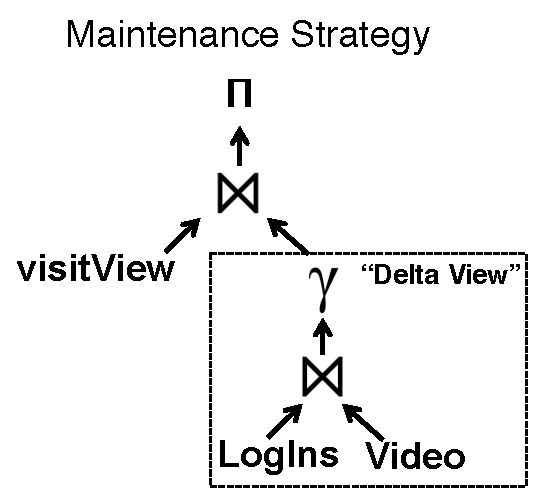
\includegraphics[scale=0.35]{figs/example_expression_tree.pdf} \vspace{-.5em}
% \caption{We illustrate the maintenance strategy of our example view, visitView, in an expression tree. \label{maintstrat}}\vspace{-1.75em}
%\end{figure}

%While, uniform sampling supports a wide variety of query types, it may have issues with queries with highly selective predicates.
%Stratfied sampling has been proposed to mitigate this problem as in the BlinkDB project \cite{AgarwalMPMMS13}.
%However, this requires that we know our query workload in advance.  
%In this paper, we do not discuss stratified sampling and will explore this further in future work.

\subsection{\svc Workflow}
%We summarize the system in Figure \ref{sys-arch} in our introduction.
In this section, we first present an overview of the \svc workflow, and then formalize two challenging problems that we address in the workflow. Formally, the workflow of \svc is:
\begin{enumerate}[noitemsep]
\item We are given a view $S$.
\item $\mathcal{M}$ defines the maintenance strategy that updates $S$ at each maintenance period.
\item The view $S$ is stale between periodic maintenance, and the up-to-date view should be $S'$.
\item \emph{(Problem 1: Stale Sample View Cleaning)} We find an expression $\mathcal{C}$ derived from $\mathcal{M}$ 
that cleans a uniform random sample of the stale view $\widehat{S}$ to produce a ``clean" sample of the up-to-date
view $\widehat{S'}$.
\item \emph{(Problem 2. Query Result Estimation)} Given an aggregate query $q$and the state query result $q(S)$, we use $\widehat{S'}$ and $\widehat{S}$ to estimate the up-to-date result.
\item We optionally maintain an index of outliers $o$ for improved estimation in skewed data.
\end{enumerate} 

\noindent\textbf{Stale Sample View Cleaning: }
The first problem addressed in this paper is how to clean a sample of the stale materialized view.
\begin{problem}[Stale Sample View Cleaning]
We are given a stale view $S$, a sample of this stale view $\widehat{S}$ with ratio $m$, the maintenance strategy $\mathcal{M}$, the base relations $\mathcal{D}$, and
the insertion and deletion relations $\partial \mathcal{D}$.
We want to find a relational expression $\mathcal{C}$ such that:
\[
\widehat{S}' = \mathcal{C}(\widehat{S},\mathcal{D},\partial \mathcal{D})
\]
Where $\widehat{S}'$ is a sample of the up-to-date view with ratio $m$. 
\end{problem}

\noindent\textbf{Query Result Estimation: }
The second problem addressed in this paper is query result estimation.
\begin{problem}[Query Result Estimation]
Let $q$ be an aggregate query of the following form \footnote{\scriptsize For simplicity, we exclude the group by clause for all queries in the paper, as it can be modeled as part of the \textsf{Condition}.}:
\begin{lstlisting} [mathescape,basicstyle={\scriptsize}]
SELECT $agg(a)$ FROM View WHERE Condition(A);
\end{lstlisting}
If the view $S$ is stale, then the result will be incorrect by some value~$c$:
\[
q(S') = q(S) + c
\]
Our objective is to find an estimator $f$ such that:
\[
q(S') \approx f(q(S),\widehat{S},\widehat{S}')
\] 
\end{problem}

\begin{example}\label{infexample}
Suppose a user wants to know how many videos have received more than 100 views.
\begin{lstlisting}[basicstyle={\scriptsize}]
SELECT COUNT(1) FROM visitView WHERE visitCount > 100;
\end{lstlisting}
Let us suppose the user runs the query and result is $45$.
However, there have now been new records inserted into the Log table making this result stale (for clarity no changes to \tbl{Video} or deletions).
First, we take a sample of \tbl{visitView} and suppose this sample is a 5\% sample.

In Stale Sample View Cleaning (Problem 1), we calculate an expression $\mathcal{C}$ based on the maintenance strategy $\mathcal{M}$ described in Example \ref{concepts},
takes the database $\mathcal{D}$ (\tbl{Log} and \tbl{Video}), and the delta relation $\partial \mathcal{D}$ (\tbl{LogIns}).
$\mathcal{C}$ is an optimized relational expression that materializes only a sample of of the updates.
In Query Result Estimation (Problem 2), we take the result of running $\mathcal{C}$ and estimate our above query.
\end{example}

\iffalse
Our query correction component takes the two corresponding samples $\widehat{S'}$ and $\widehat{S}$, and calculates a correction to~$q(S)$.

Like similar restrictions in other sample-based systems \cite{agarwalknowing}, there are restrictions on the queries $q$ on the view that we can answer. 
In the SampleClean work, we focused on \sumfunc, \countfunc, and \avgfunc queries of the form\footnote{\scriptsize For simplicity, we exclude the group by clause for all queries in the paper, as it can be modeled as part of the \textsf{Condition}.}: 
\begin{lstlisting} [mathescape,basicstyle={\scriptsize}]
SELECT $f(a)$ FROM View WHERE Condition(A);
\end{lstlisting}
In this work, we expand the scope of the query processing, and consider general non-nested aggregate queries with predicates.

We also consider correcting stale non-nested select queries of the following form with predicates:
\begin{lstlisting} [mathescape,basicstyle={\scriptsize}]
SELECT * FROM View WHERE Condition(A);
\end{lstlisting}
As with all sample estimates, the accuracy increases with sample size, thus less selective predicates lead to more accurate results.




Note, that this definition is slightly different from the reservoir sampling techniques studied in AQP \cite{DBLP:journals/toms/Vitter85} which find a uniform sample of fixed \emph{size} $k\le \mid S \mid$.
Our sampling ratio gives a sample of the size $k$ in expectation, however, the actual size from any given instance may be slightly different.
For large sample sizes, there is little difference between the techniques since the actual size of using a sample ratio will be close to $k$.
The uniform sample model represents our algorithm which uses hashing better and also makes the presentation of our analysis more clear.

Furthermore, any ``black-box'' uniform sampling algorithm can be used to achieve a reservoir sample.
The use of one technique over another does not affect the general principles or the statistics of \svc, only the 
notation in the analysis.


%\vspace{2em}
\subsection{Problem Statements}
\subsubsection{View Maintenance as Data Cleaning}\label{cleaning}
%In \svc, we model staleness in an MV as a type of data error.
We formalize the problem of correcting staleness as a data cleaning operation so we can apply our data cleaning approach.
In the unsampled case, $\mathcal{M}$ defines a data cleaning operation.
If we are given a materialized view $S$ and we know the base relations have had insertions and deletions, then there are three possible types of error:
(1) a row in $S$ needs to be updated, (2) a row in $S$ needs to be deleted, and (3) new row needs to be inserted into $S$.
Applying $\mathcal{M}$ removes these errors making the view ``clean".
%In the absence of these errors, we call a view \emph{up-to-date}.

However, now suppose we have a sampled view $\widehat{S}$, simply applying updates to the rows in the sample may not suffice.
If new rows need to be inserted into $S$, those will never be represented in the sample violating our uniform sampling.
Thus, we define cleaning in the following way: suppose we have a stale uniform sample $\widehat{S}$, cleaning this sample
should give us $\widehat{S'}$ a uniform sample of the up-to-date view $S'$ with the same sampling ratio.
Formally, this can be represented as the following operations: (1) if an update is needed, update the row, (2) if a row needs to be deleted, delete the row, and (3) for all new rows that need to be inserted into the view $S$ insert a random sample of ratio $m$.

Due to the insertions, the defined data cleaning on a sample does not necessarily give a unique $\widehat{S'}$, so the next question is how to formalize the link between $\widehat{S}$ and $\widehat{S'}$. 
To link a corresponding stale sample (dirty data) and up-to-date sample (clean data), we define the following property:
\begin{definition}[Correspondence]
$\widehat{S'}$ and $\widehat{S}$ are uniform samples of $S'$ and $S$, respectively.  We say $\widehat{S'}$ and $\widehat{S}$ correspond if and only if:
\vspace{-.25em}
\begin{itemize}[noitemsep]
\item For every row $r$ in $\widehat{S}$ that required a delete, $r \not\in \widehat{S'}$
\item For every row $r$ in $\widehat{S}$ that required an update to $r'$, $r' \in \widehat{S'}$
\item For every row $r$ in $\widehat{S}$  that was unchanged, $r \in \widehat{S'}$
\item For every row $r$ in $S$ but not in $\widehat{S}$, $r \not\in \widehat{S'}$
\end{itemize}
\vspace{-.25em}
%\item For every row $r$ in $S'$ that is newly inserted, $r \not\in \widehat{S}$.
%\item If a row $r$ requires an update and then a deletion. The deletion takes precedence and $r \not\in \widehat{S'}$.
%\item Rows that are inserted trivially satisfy the conditions since those rows are not contained in $S$ or $\widehat{S}$.
\label{correspondence}
\end{definition}
%This definition of correspondence gives us a way to get two samples from which we can take a row-by-row difference.
%There is some nuance in how to handle null values which we discuss in Section \ref{correction}.

The goal of \svc is to efficiently produce a corresponding up-to-date sample from a stale one thus cleaning the sample.
In the first component of \svc (Section \ref{sampling}), we take as input a uniform sample of a stale view $\widehat{S}$, a maintenance strategy $\mathcal{M}$, and a set of updates $\{\Delta R_i\} \cup \{\nabla R_i\}$.
We return $\widehat{S'}$, a clean uniform sample (a uniform sample of $S'$) that satisfies the correspondence property with $\widehat{S}$.

\iffalse

\begin{example}[Correspondence]
Suppose \tbl{countView} has 4 video rows: 
\begin{lstlisting} [mathescape]
V1 (visitCount = 4), V2 (visitCount = 6), V3 (visitCount = 1), V4 (visitCount = 1)
\end{lstlisting}
We take a sample of \tbl{countView} and call it \tbl{countViewSample} that contains V1 and V2.
\tbl{LogIns} has new logs of 1 visit for V1 and 1 visit for a new video V5.
An up-to-date sample that corresponds is:
\begin{lstlisting} [mathescape]
V1 (visitCount = 4+1), V2 (visitCount = 6)
\end{lstlisting}
An up-to-date sample that does \emph{not} corresponds is: 
\begin{lstlisting} [mathescape]
V1 (visitCount = 4+1), V3 (visitCount = 1)
\end{lstlisting}
This is because V2 was unchanged and therefore should be included in the sample.
\end{example}
\fi

\subsubsection{Query Result Correction}
In the query result correction phase, we take a query result on a stale view and use the up-to-date sample to compensate for the staleness.
Given a query $q$ which has been applied to the stale view $q(S)$ giving a stale result.
Our query correction component takes the two corresponding samples $\widehat{S'}$ and $\widehat{S}$, and calculates a correction to~$q(S)$.

Like similar restrictions in other sample-based systems \cite{agarwalknowing}, there are restrictions on the queries $q$ on the view that we can answer. 
In the SampleClean work, we focused on \sumfunc, \countfunc, and \avgfunc queries of the form\footnote{\scriptsize For simplicity, we exclude the group by clause for all queries in the paper, as it can be modeled as part of the \textsf{Condition}.}: 
\begin{lstlisting} [mathescape,basicstyle={\scriptsize}]
SELECT $f(a)$ FROM View WHERE Condition(A);
\end{lstlisting}
In this work, we expand the scope of the query processing, and consider general non-nested aggregate queries with predicates.

We also consider correcting stale non-nested select queries of the following form with predicates:
\begin{lstlisting} [mathescape,basicstyle={\scriptsize}]
SELECT * FROM View WHERE Condition(A);
\end{lstlisting}
As with all sample estimates, the accuracy increases with sample size, thus less selective predicates lead to more accurate results.
%From these queries, we exclude the group by clause, as we model group by clauses as part of the \textsf{Condition}.
\fi

\iffalse
\subsubsection{Outlier Indexing}
The query correction in the previous subsection is derived from a sample.
Sampling is known to be sensitive to outliers, which we define as records whose values deviate significantly from the mean.
However, a challenge is that since we do not materialize the entire up-to-date view detecting which records may be outliers is challenging.
Instead, we define an outlier index on base relations of the database $\mathcal{D}$.
This index tracks records whose attributes cross some threshold $t$.
Then, for a given view $S$, this component gives a series of rules to propagate the information from the outlier index upwards.
Basically, for every row in the view that is derived from a record in the outlier index, we ensure that it is incorporated into the sample.
We use the set of outliers to return a more accurate correction result.
\fi
%We explore the conditions under which we can make this guarantee, and discuss query processing with the outlier index in Section \ref{outlier}.


\iffalse
\subsection{Example Application}
Returning to our example \tbl{countView}, suppose a user wants to know how many videos have received more than 100 views.
\begin{lstlisting}[basicstyle={\scriptsize}]
SELECT COUNT(1) FROM visitView 
WHERE visitCount > 100;
\end{lstlisting}
Let us suppose the initial query result is $45$.
There now have been new log records inserted into the Log table making the old result stale.
For example, if our sampling ratio is 5\%, that means for 5\% of the videos (distinct \tbl{videoId}), we update just the view counts of those videos.
Suppose 2 videos have changed their counts from less than 100 to greater than 100.
%From this sample, we calculate how many new videos changed from less than 100 views to times greater than 100; let us suppose this answer is $2$.
%Since our sampling ratio is 5\%, 
From this sample, we extrapolate that $40$ new videos throughout the view should now be included in the count.
This means that we should correct the old result by $40$ resulting in the estimate of $45+40 = 85$.
\fi


%\subsection{Logical Operators}
\projx specifies three logical operators: Extraction, Filtering, and Similarity Join. 
\sanjay{In depth why these operators are {\it sufficient}.}

For performance (or some other reason), we support several additional
logical operators tha enable optimization: Sampling, Async, and Transitive Closure.
The composition of these operators support a variety of data cleaning
operations. 
For example, a deduplication task can be expressed as a Similarity Join to pair similar records
together and then a filtering task to remove false positives.
These logical operators specify the input and output data schema and allow us to compose operations.


\vspace{0.5em}

\noindent \textsf{SimilarityJoin(R,S,$\phi$, $t$)}: For a given relations $R(a_1,...,a_l)$ and $S(b_1,...,b_k)$, a similarity function $\phi$, and a threshold $t$, the similarity join of R and S is defined by:
\[
\{ (r,s) \in R \times S \text{ s.t } \phi (r,s) \ge t \}
\]

\vspace{0.5em}


\noindent \textsf{Filter(R, $\rho$)}: For a given relation $R(a_1,...,a_l)$ and a boolean condition $\rho$, return $R' \subseteq R$ that satisfies $\rho$.

\vspace{0.5em}

\noindent \textsf{Extract(R, a, $\epsilon$)} For a given relation $R(a_1,...,a_l)$, a attribute $a$, and an extraction function $\epsilon$, apply $\epsilon$ to every $R(a)$ returning $\epsilon(R(a)) = (v_1,...,v_k)$. The result relation is:
\[
R(a_1,...,a_l,\epsilon(R(a)))
\]

\noindent \textsf{Sample(R, $m$)}: For a given relation $R(a_1,...,a_l)$ and return $R' \subseteq R$ such that each $r \in R$ is in $R'$ with probability $m$.

\vspace{0.5em}

\noindent \textsf{Project(R, $p_1,...,p_k$)}: For a given relation $R(a_1,...,a_l)$ and return $R(p_1,...,p_k)$.

\vspace{0.5em}

\noindent \textsf{TransitiveClosure(R,$f$)}: For a given relation of pairs of rows from the same base relation, e.g the result of a self-Similarity Join, $R(a_1,...,a_l, b_1,...,b_l)$ return the transitive closure of the relation $S(a_1,...,a_l)$. $f$ is called a cannonical representation function, this takes a set of associated records and returns a single record that is designated as the canonical representation.






%\section{Physical Operators and Implementation}

For each of the logical operators there are different physical implementations.
We do not currently select the appropriate physical operator and the user has to specify this.
We do, however, set sensible default parameters for each of the physical operators.
In \projx, there are three broad categories of physical operators: Automated, Crowd, and Learning.
An automated physical operator is conceptually the same as a SQL user defined function, while a crowd operator uses a microtask platform.
A learning operator takes in training examples (whether crowd or ground truth) and learns an automated operator.
We describe each below.

\ewu{below are straightforward physical implementations of the
logical operators.  Is there anything interesting to say about their
design or a specific physical operator?}

\team{How do we know when transitive closure/any of the physical operators can be safely applied?  Are there properties of the physical ops that could tell us?}


\subsection{Similarity Join} 
\projx provides a library of the following commonly used similarity functions: \textsf{JaccardSimilarity}, \textsf{DiceSimilarity},
\textsf{CosineSimilarity}, \textsf{OverlapSimilarity}, and \textsf{EditDistance}.
The user can select one of these similarity functions.
A naive implementation of a Similarity Join is to take the cartesian product and then filter all pairs of record of similarity greater than $t$.
However, the implemented similarity functions are all symmetric and the similarity function is maximized when $r = p$.
So it suffices to compute a similarity $\theta$-join instead of the full Cartesian product.
We can further add an optimization called prefix filtering to further reduce the number of similarity function evaluations.
In prefix filtering, we prune pairs that cannot possibly meet the threshold $t$ based on the number of tokens that overlap which can be determined with an inverted index.


\subsection{Extraction}
We implement basic automated extraction libraries including delimited splitting and regular expression methods.
However, extraction is a task that is well suited for crowd sourcing.
We provide a parametrized interface that allows the user to specify an extraction attribute, a formatting question, and request data from the crowd.
In Figure \ref{fig:entry}, we illustrate an example of this task.

\begin{figure}[ht!]
\centering
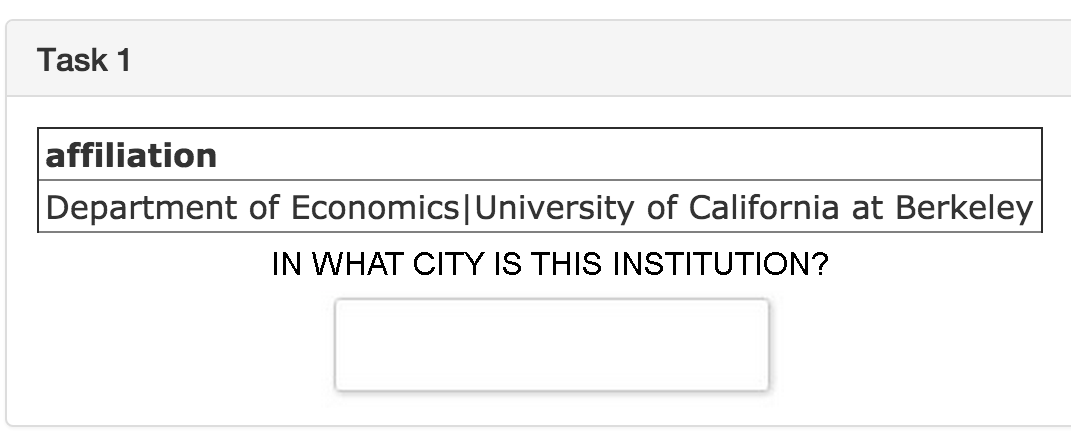
\includegraphics[scale=0.25]{figs/entry.png}
\caption{Example of the Extraction Crowd Interface. \label{fig:entry}}\vspace{-.5em}
\end{figure}

\subsection{Filtering}
We provide an interface for a user defined predicate.
However, as with extraction, filtering has many opportunities for crowdsourcing.
For a filtering operation, the crowd response is binary in contrast to Extraction.
We provide crowd templates for two types of filtering tasks.

\noindent\textbf{Condition Checking: } Given a single record, a crowd worker indicates if it satisfies some condition. In Figure \ref{fig:condition},
we illustrate an example condition checking task.
\begin{figure}[ht!]
\centering
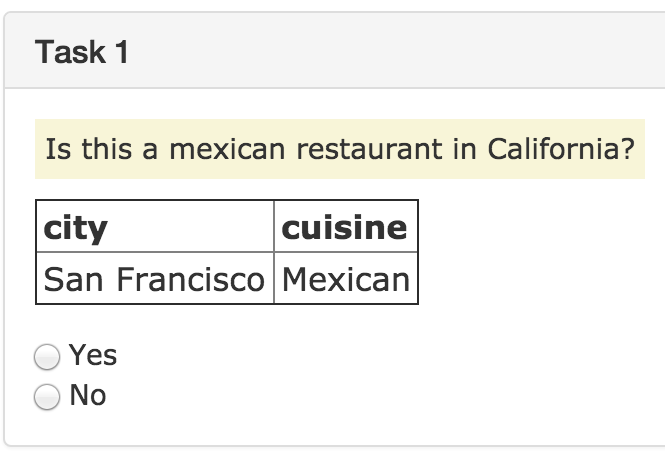
\includegraphics[scale=0.25]{figs/condition.png}
\caption{Condition checking is one variant of the filtering crowd interface.\label{fig:condition}}\vspace{-.5em}
\end{figure}

\noindent\textbf{Pair Comparison: } Given a pair of records, a crowd worker indicates if they are the same or are different. In Figure \ref{fig:pair},
we illustrate an example pair comparison task.

\begin{figure}[ht!]
\centering
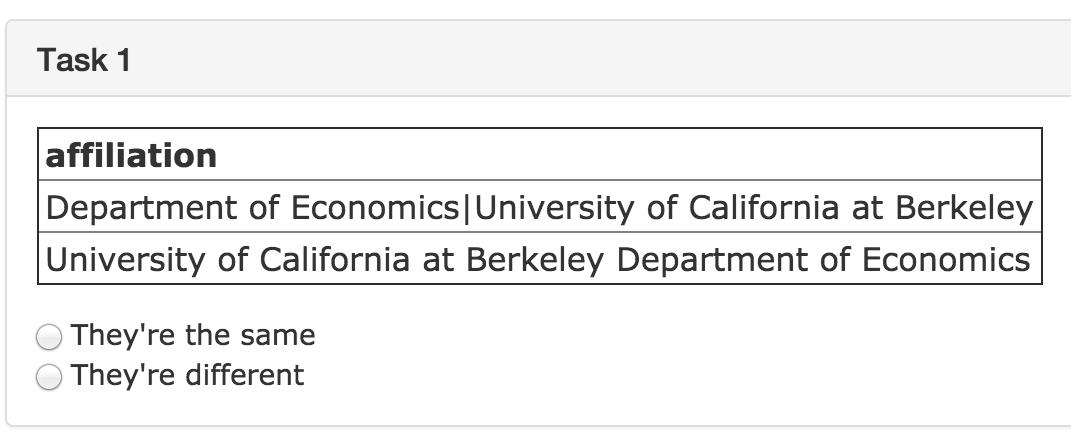
\includegraphics[scale=0.25]{figs/pair.png}
\caption{Pair comparison is the other variant of the filtering crowd interface.\label{fig:pair}}\vspace{-.5em}
\end{figure}



\subsection{Extended Operators}

\subsubsection{Sampling}
\projx provides different variants of uniform sampling.
We provide Bernoulli sampling (in which flips a ``biased coin" for each row) or hash sampling (which hashes an attribute).
Hash sampling allows for joining sampled relations with foreign key relationships.
On the other hand, Bernoulli sampling is less sensitive to skews and leads to more consistent sample sizes.

\subsubsection{Transitive Closure}
Similarity Joins can create issues with transitivity.
For example, rowA might be similar to rowB and rowB might be similar to rowC, but rowA might not be similar to rowC.
We can associate these relationships with edges in a similarity graph.
Then to enforce transitive closure, we solve a connected components problem.
We apply a distributed using a distributed gather-apply-scatter connected components algorithm in the Spark-integrated graph library GraphX.




% %!TEX root = demo.tex
\section{Logical Operators}


\ewu{INSERT: implementation in Spark}

Now, we discuss the logical operators and their parameterization defined in \projx.

\vspace{1em}


% !TEX root = demo.tex
\section{Research Challenges}
To support evolving data quality needs, there are three main research challenges in \sys: (1) sampling, (2) recommendation, and (3) crowd sourcing.

\subsection{Sampling}
In prior work, we explored the problem of estimating aggregate query results over dirty data ~\cite{wang1999sample, svc}.
In SampleClean \cite{wang1999sample}, we found that aggregate queries can often be answered with very high accuracy (i.e 99\%) with only a small fraction of clean data, and we can clean just enough for the application's data quality requirements.
In \sys, we implement sampling as a logical operator that can be used for quickly prototyping and optimizing workflows on samples of data and then transferring these optimizations to full datasets.
We find that many important features of iterative data cleaning workflows can be posed as aggregate queries on samples with confidence intervals.
If we want to know whether a data cleaning operation has a significant effect, we can use a query to test the effects of this operation on a sample.
For example, if we are deduplicating restaurant categories, we can count the number of Chinese restaurants in a sample to test if different deduplication algorithms significantly affect the count.
Sampling and result estimation are salient features of \sys that allow us tune parameters and provide recommendations for chaning a workflow without evaluating all possible workflows on the full data.
Next, we discuss how we can efficiently generate these recommendations.

\subsection{Recommendation}
We also have implemented a basic recommendation engine that recommends changes to a data cleaning plan based on user feedback. 
A user can specify a set of ground truth tuples, and our system will optimize over data cleaning plans that best reproduce the ground truth.
There are three types of recommendations: (1) parameter change, (2) operator replacement, and (3) operator addition.
To realize and execute the recommendations, we use caching and lineage to efficiently re-evaluate a workflow.

\vspace{.4em}

\textit{Parameter Change.} Many of the physical operators in \sys have tunable parameters, whose values are often very dataset-specific, and the user feedback gives us a way to evaluate the quality of the initial parameter choice. 
For example, Similarity Joins have a similarity threshold and a similarity function. 
Increasing this threshold reduces the selectivity of the join, and \sys needs to choose a threshold that maximizes accuracy. 
This problem can be solved by a minimum-cost spanning tree over a similarity graph (edges represent non-zero similarity) over tuples.

\vspace{.4em}

\textit{Operator Replacement.} 
\sys recommends changes to physical operators when the user indicates that they are not satisfied with the output.
For example, we can treat user feedback as a proxy for crowd labels and estimate the value of replacing a physical operator with an active learning variant.
Additionally, we can try different variants of automated operators to test how accurate they are with respect to the user feedback.

\vspace{.4em}

\textit{Operator Addition.}  There are also cases where we may want to add another physical operator, while still preserving the logical input-output behavior of the workflow.
It is common in extraction tasks to have most tuples accurately extracted with an automated extractor but only a small subset requiring additional inspection. 
For these cases, we can add a crowd-based \textsf{Filter} operator to separate these examples for additional cleaning.

\vspace{.4em}

\textit{Cost Estimates.} Of course, changing plans when using crowdsourcing may significantly change its cost.
For every recommendation, we estimate the number of additional tuples processed by the crowd operators and provide the user with an estimated cost.
Based on a user-specified cost per task, we estimate the number of tasks needed to clean the dataset.

\vspace{.4em}

\textit{Caching} allows for result re-use if a downstream operator is modified or added.
If the system has sufficient memory, then we can na\"{\i}vely cache all intermediate results. 
Otherwise, the key challenge is to select a subset of results to cache.
We choose which results to cache by integrating the caching framework with our recommendation engine.
When we make a recommendation for a change, we must cache the preceding operator. 

\vspace{.4em}

\textit{Lineage} allows us to understand how results change if upstream operators are modified.
For example, decreasing a similarity join threshold increases the number of output pairs without affecting existing output pairs. The key property here is monotonicity, and some types of monotone \textsf{Filter} and \textsf{SimilarityJoin} operators are data cleaning analogs for a Select-Join relational algebra.
We can therefore model upstream hot-swapping as an incremental view maintenance problem and update the 
final result based on the insertion or deletion of tuples earlier in the plan.

\iffalse
\vspace{.5em}



\fi

%\subsubsection{Dynamic Modification}
%The next category of optimizations happen at the plan-level, i.e., the sequence or execution pattern of the operators.
%We highlight two challenges: allowing users to see early results, and allowing users to modify plans mid-execution.
%\vspace{.3em}
%{\noindent \bf Asynchronous Data Cleaning:} To provide fine-grained feedback during a data cleaning process, our system executes data cleaning operations asynchronously. Tuples are processed in a streaming fashion by each of the operators in the plan and the intermediate results are persisted, allowing users to query the results at any time. Thus, at any time, the user can get a ``best effort" query result.
%\vspace{.3em}


%\vspace{-0.2cm}
\subsection{Crowdsourcing}
%\vspace{.2em}

%{\noindent \bf Sampling:} One way to reduce operator latency is to reduce the number of tuples each operator processes.
%In \sys, sampling is a first-class logical operator that can be used for quickly prototyping and optimizing workflows on samples of data and then transfering these optimizations to full datasets.
%Sampling allows for quick introspection of otherwise opaque components, such as testing the quality of a crowd with a small set of tuples.
%\sys also provides the statistical tools to extrapolate (with confidence intervals) the insights learned on a sample.
%The problem of estimating aggregate query results over dirty data has been investigated in prior work~\cite{wang1999sample}, 
%addressing the challenge that data cleaning may change the underlying statistics of a sample.
%In this work, we build on these results to allow users to declare aggregate queries of interest and notify them when a change to 
%a plan has a statistically significant effect.

%Recently proposed, sample-based query processing methods for dirty data can help inform users the changes about the statistical significance of 
%changes made to the data.
%For example, suppose one collects a restaurant dataset, and runs some aggregation queries on the dataset, e.g., computing the number of the restaurants in San Fransisco and getting a query result of 12000. 
%But, when looking at the dataset, she finds that there are many duplicate restaurants in the dataset, and some restaurants' locations are misspelled (e.g., S\underline{e}n Fransisco). She can use our system to create a sample of the data, and then apply a data cleaning procedure to the sample. 
%After the sample is cleaned, our system can estimate the impact of data cleaning on her original query results, and return her corrected answers with confidence intervals, e.g., $5000\pm300$. Intuitively, this result means that if the same data-cleaning procedure is applied to the full dataset, the number of the restaurants in San Fransisco will be within $[4700, 5300]$. 

%\vspace{.5em}
%{\noindent \bf Crowdsourcing and Active Learning:} 
Working with crowds is inherently challenging.
Unlike when using automated operators, the accuracy and speed of processing each tuple varies widely with the crowd worker assigned to it.
Completion time of an operator depends on the response times of individual workers, and on real-world crowdsourcing 
platforms, the distribution of response latencies is highly skewed; analogous to the straggler problem in distributed systems.
We address this problem by maintaining a pool of high-speed, high-quality crowd workers and develop task routing strategies 
that can avoid assigning tasks to slow workers and leverage redundancy to significantly reduce the time that is required to clean 
data with the crowd. 
Additionally, active learning techniques reduce the number of tuples that require crowd work to clean the data.
%Even cleaning a sample of data, data cleaning can still take a lot of time. This is especially true when it requires humans to clean the data. 

\vspace{-0.25cm}


\iffalse
\subsection{Research Challenges}

Architecturally, we separate crowd sourcing and automated data cleaning.
There is a crowd server that acts as a layer of indirection between the Spark codebase and crowd sourcing APIs.

\team{Describe Research Challenges.  To what extend can we actually do
optimization given the physical operators?  Unlike relalgebra, the physical operators here are
not interchangable!}



\subsection{Learning Parameters From Example}
In simple cases, it might be easy to use domain knowledge to select and tune physical operators. 
In more complex cases, it might be easier to specify a sample of dirty and clean data instead of the function.
It may also not be feasible to have the crowd clean the entire dataset.
In these cases, we want to learn a statistical model from which we can extrapolate those responses to the rest 
of the data.

In our current implementation of \projx, we pose this learning problem as classification problems.
In general, these parameter functions can be quite complex and this is a simplification of the learning problem.
The choice of classifier and featurization is upto the user. 
We currently support Support Vector Machines and Decision Trees with a featurization library that includes common text processing features.

\vspace{0.5em}

\noindent \textsf{Filter(R, $\mathcal{T}^+$, $\mathcal{T}^-$)}: Given a set of positive training examples $\mathcal{T}^+$ (i.e, $r$ that satisfy the condition) and
negative training examples $\mathcal{T}^-$ (i.e, r that do not satisfy the condition), we learn a classifier that predicts whether a tuple satisfies the condition. 

\vspace{0.5em}

\noindent \textsf{Extract(R, a, $\mathcal{T}$)} We restrict the learned problem setting to delimited extraction. Given a set of training examples $R(a)$ and the output $v_1,v_2,...,v_k$, we learn a classifier to predict which characters in $R(a)$ are delimiters based on the tokens in the string.

\vspace{1em}

To acquire the samples of clean data, uniform sampling may not be the best strategy.
For example, if there examples of dirty data are very rare, we will not be able to learn a model.
We implement a technique called Active Learning to sample.
Active Learning selects the most informative examples based on the current model so far.
We use an Active Learning algorithm called uncertainty sampling to do this.




\subsection{Inspection}

Data cleaning requires inspection -- user wants to see how the dataset
has been "cleaned"  through the pipeline.  What does that even mean?

\subsection{Dynamic Re-optimization}

Crowd means want to swap in or out operators at run time.


\subsection{Lineage}

\noindent\textbf{Lineage: }
We track the lineage of rows using a primary key.
Users are not allowed to modify this primary key with any operations.
This allows us to apply operations like transitive closure even after projection since we have a unique identifier for each row.

\vspace{0.5em}
\noindent \textbf{Example: } Suppose, we are interested in deduplication of unstructured data. Then, we could apply the following logical operations.
We first apply an \textsf{Extract} operation to extract the unstructured data into columns. If some of the columns are inconsistent in their representation,
we apply \textsf{Project} to those columns that are inconsistent. We can then take a \textsf{SimilarityJoin} to group rows that are similar, and finally
we resolve those differences with \textsf{TransitiveClosure}.
\fi



% !TEX root = demo.tex
\subsection{Engineering Challenges}
In addition to the numerous research challenges, there have been substantial challenges in engineering \sys.
We highlight two key challenges: API design and Crowdsourcing.

\subsubsection{API Design}
Currently, there are many systems that address specific types of data error \cite{gokhale2014corleone,park2014crowdfill,eracer,chen2014integrating}, but it is often 
the case that data are corrupted in multiple ways.
Unfortunately, there is currently no interoperability between these systems, since some are constraint-based, some use generic crowd APIs, and others have custom crowd interfaces.
In \sys, we address this problem by designing an API that allows for the composition and optimization of data cleaning operators.
Many of the research challenges in \sys rely on clear specifications of the input and output behaviors of
individual data cleaning operators.
For example, Hot Swapping is only possible between two physical operators that have exactly the same input and output specification.
The engineering challege is to retain modularity and extensibility while restricting operators.
We build a class hierarchy of data cleaning operators which through inheritance and parameterization specify clear input and output behaviors.

One draw back of an extensive API is that the choices may overwhelm a user.
Many of our API methods and classes come with inherited sensible defaults.
For example, if the user fails to completely specify the semantics of the similarity function through the API, 
the system will avoid optimizations and perform a naive cartesian products and filtering.
These behaviors come naturally through the use of inheritance and polymorphism.

\subsubsection{Crowdsourcing Platform}
The second engineering challenge is designing a platform to serve crowd tasks.
Working with crowds is inherently challenging: unlike with automated operators, the accuracy and speed of processing each tuple varies widely with the crowd worker assigned to it.
We have developed a ``crowd manager" as a layer of indirection to support this complexity.
This component handles serving and processing crowd tasks and automatically uses our techniques for latency reduction as well as state-of-the-art quality control techniques using redundancy and Expectation-Maximization based voting algorithms.

The other benefit of a crowd manager is that it provides an abstraction layer over the varied APIs of Mechanical Turk, Crowd Flower, and others.
We leverage the fact that most crowd platforms serve tasks through a browser-based interface, generating tasks in the form of dynamic web pages and processing responses via AJAX callbacks to our own server.
As a result, tasks submitted to the crowd manager can be processed easily on a variety of different crowds including AMT, Crowd Flower, or a private ``Internal Crowd".
%\input{implementation.tex}
%\section{\projx DSL}
We design a DSL for the composition of data cleaning operations.
The general syntax of this language is:
\begin{lstlisting}
<logical operator> on <relations>
	with <physical operators> , <params>
\end{lstlisting}
In this section, we will highlight some key examples.
We have an additional operator \textsf{Async} which designates the 
execution of the operator to be synchronous or asynchronous.

\subsection{String Extraction}
One of the most common data cleaning operations is delimited extraction.
In our DSL, this can be expressed in the following way:
\begin{lstlisting}
Extract on Data
with Split, `,',
cols=[col1, col2]
\end{lstlisting}

We can also use a format string:
\begin{lstlisting}
Extract on Data
with FmtString, `%s:%s',
cols=[col1, col2]
\end{lstlisting}

\subsection{Crowd Entity Resolution}
Crowd-based techniques for entity resolution are increasingly popular e.g Corleone \cite{DBLP:conf/sigmod/GokhaleDDNRSZ14}.
We present an example of expressing a crowd-based technique for entity resolution with the DSL.
Let us suppose we have a database of addresses that we want to deduplicate.
The first step is to group similar rows together and a good similarity metric to use is JaccardSimilarity.
\begin{lstlisting}
SimilarityJoin on Data
with Jaccard, thresh=0.8
\end{lstlisting}
The next step is to filter these pairs using the crowd. 
However, since most pairs will not be duplicates we want to use Active Learning.
Furthermore, since the crowd might be slow, we can add asynchrony.
\begin{lstlisting}
Filter on
( 
 SimilarityJoin on Data
 with Jaccard, thresh=0.8
)
with Crowd, Active, Async
\end{lstlisting}
To resolve the changes, we apply transitive closure at the end that takes the 
longest address:
\begin{lstlisting}
TransitiveClosure (
 Filter on
 ( 
  SimilarityJoin on Data
  with Jaccard, thresh=0.8
 )
 with Crowd, Active
) with Longest
\end{lstlisting}




% !TEX root = demo.tex
\section{Demonstration}
In this section, we detail the proposed demonstration.
The objective of this demonstration is to illustrate 
how \sys enables the rapid iterative construction of data cleaning plans
and the ability to transfer workflows between similar dirty datasets.

\subsection{Datasets}
In the demo, we will consider cleaning workflows on three different datasets.
The first dataset contains 858 Zagat reviews\footnote{\scriptsize{ \url{cs.utexas.edu/users/ml/riddle/data/restaurant.tar.gz}}},
each tagged with the cuisine of the restaurant reviewed (e.g. ``Chinese" or ``French").
The second dataset, which is similar to the first, is from Yelp \footnote{\scriptsize{\url{https://www.yelp.com/academic_dataset}}} and contains 58,127 restaurant records that are also tagged with a category.
The third dataset consists of $3,049,914$ records of liquor sales from the state of Iowa\footnote{\scriptsize{\url{data.iowa.gov/Economy/Iowa-Liquor-Sales/m3tr-qhgy}}}, including the store where the purchase occurred and the items and cost of the purchase.
In all three datasets, categorical columns are inconsistent across records (e.g. cuisine tags for ``Chinese" vs. ``Chinese Cuisine"), records are duplicated, and formatting errors abound. 
We will use \sys to resolve these errors using Extraction and Entity Resolution, then run aggregate queries over the cleaned datasets.

\begin{figure}[t]
\centering
 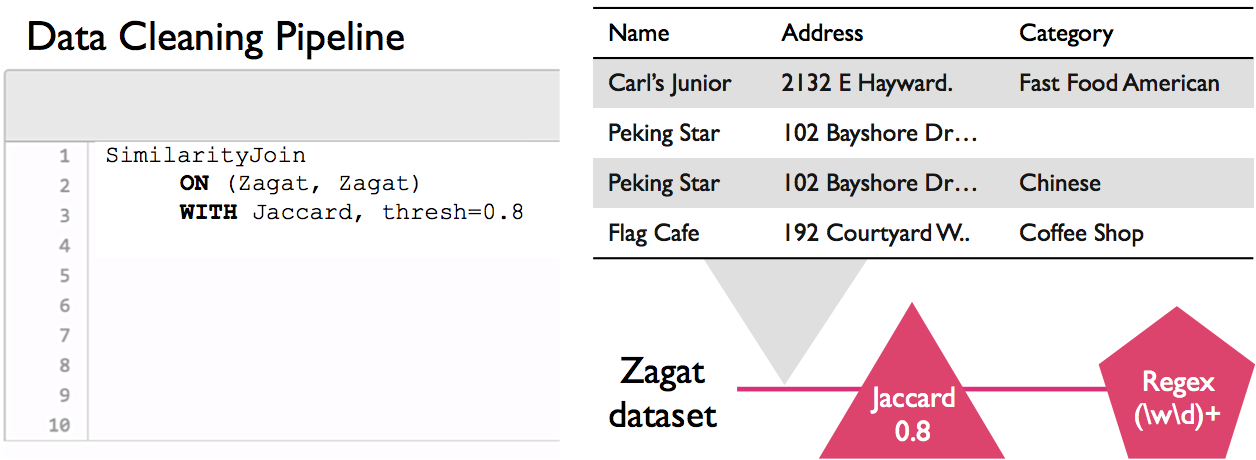
\includegraphics[width=\columnwidth]{figs/dashboard_screenshot.png}
 \caption{The dashboard contains both a visual interface and a text box to specify data cleaning operations. When the user is satisfied, she can run the plan and see the results on the right. \label{screenshot}}
\end{figure}


\begin{figure}[t]
\centering
 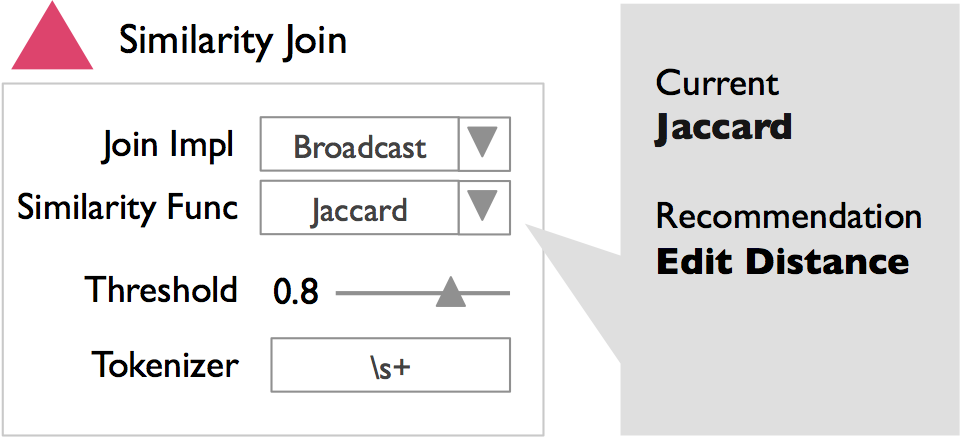
\includegraphics[width=0.8\columnwidth]{figs/dashboard_recsys.png}
 \caption{The operator view lists the parameters of an operator. Users can view recommended changes and modify parameters on the fly.}
 \label{screenshot-rec}
 \vspace{-0.4cm}
\end{figure}

\subsection{Demo Walkthrough}
Below, we detail the steps of the proposed demonstration.
A screenshot of the dashboard interface is illustrated in Figure~\ref{screenshot}.

\vspace{0.2em}

\noindent\textbf{Step 1: } Participants will select a dataset (e.g., the Zagat dataset), and load a pre-populated data cleaning plan and target query for it.
Participants must first extract the columns of the dataset into the proper schema using a regex-based Extraction.
Then, participants will be able to manually tune the Enity Resolution by choosing between Similarity Join implementations, adjusting the thresholds for the Similarity Join, and adding a crowdsourced filtering step.

\vspace{0.2em}

\noindent\textbf{Step 2: } At all times, the interface will display a representative sample of the cleaning plan's input and output and the results of the target query so that the participant can see how cleaning affects the data. 
If a plan modification adds crowdsourcing, participants can complete crowd tasks in \sys's crowd interface.

\vspace{0.2em}

\noindent\textbf{Step 3:} Participants re-evaluate and adjust their plan by clicking on an operator (Figure~\ref{screenshot-rec}).
This view will show the system's recommended changes to the operator and allow the participant to make those changes easily.
For example, Figure~\ref{screenshot-rec} shows a recommendation to change the similarity metric from Jaccard to Edit Distance since the attribute in question does not have many tokens.

\vspace{0.2em}

\noindent\textbf{Step 4: } Participants can then switch datasets. Switching between restaurant datasets (Zagat and Yelp) demonstrates reuse of the same plan on novel data, while switching to the alcohol dataset demonstrates that \sys is effective across data domains.

%\section{Conclusion}
In this demonstration, we present a prototype of our \projx system.
Our demonstration concludes with the following take-away messages:
(1) It is beneficial to have an integrated data cleaning solution in the analytics stack,
(2) \projx is a general purpose system that implements many of the salient features of sample-and-clean and progressive data cleaning frameworks, and
(3) the API is concise and intuitive to use.

\section{Acknowledgments}
This research is supported in part by NSF CISE Expeditions award CCF-1139158 and DARPA XData Award FA8750-12-2-0331, and  gifts from Amazon Web Services, Google, SAP,  Apple, Inc., Cisco, Clearstory Data, Cloudera, Ericsson, Facebook, GameOnTalis, General Electric, Hortonworks, Huawei, Intel, Microsoft, NetApp, Oracle, Samsung, Splunk, VMware, WANdisco and Yahoo!.













{
\bibliographystyle{abbrv}
\fontsize{8pt}{9pt} \selectfont
\bibliography{refs/bigdata}
}



\end{document}
